\section{Pandas}\label{sec:08-pandas}

\subsection{DataFrame-Grundlagen}\label{sec:08-dataframe-grundlagen}
\ZSFindex{Pandas}
\ZSFindex{DataFrame}
\subsubsection{DataFrame erzeugen}\label{sec:08-dataframe-erzeugen}
\begin{contentbox}
\CodeLine{import pandas as pd}\\
\CodeLine{df = pd.DataFrame()}[leerer DataFrame]\\
\CodeLine{df = pd.read_csv("Name.csv")}[DataFrame aus CSV laden]
\end{contentbox}

\subsubsection{Zeilen/Spalten auswählen (loc / iloc)}\label{sec:08-auswählen}
\ZSFindex{loc}
\ZSFindex{iloc}
\begin{contentbox}
\CodeLine{data["Month"]}[einzelne Spalte]\\
\CodeLine{data[["Name", "City"]]}[mehrere Spalten]\\
\CodeLine{data["Name"][2]}[gibt `Carlos' zurück]\\
\ZSFgapS
\CodeLine{data.iloc[1]}[Zeile mit Index 1]\\
\CodeLine{data[1:3]}[Zeilen mit Index 1 und 2]\\
\CodeLine{data.loc[1:3, "M":"C"]}[Zeilen 1--3, Spalten M bis C]\\
\CodeLine{data.iloc[1:3, 0:2]}[wie loc, aber indexbasiert]
\end{contentbox}

\subsubsection{Zeilen filtern (Bedingung / boolean mask)}\label{sec:08-filtern-von-zeilen}
\begin{contentbox}
\CodeLine{data[data["Age"] > 30]}[alle Personen über 30]\\
\CodeLine{data["Name"][data["Age"] > 30]}[nur Namen dieser Personen]
\end{contentbox}

\subsection{Daten verändern und bereinigen}\label{sec:08-daten-veraendern-und-bereinigen}
\subsubsection{Index \& Spalten umbenennen}\label{sec:08-spalten-umbenennen}
\begin{contentbox}
\CodeLine{data.set_index("Row")}[setzt `Row' als Index]\\
\CodeLine{data.rename(columns={"City": "Location"})}[Spalte umbenennen]\\
\CodeLine{data.columns = ["Monat", "Name", "Stadt", ...]}[jede Spalte umbenennen] % chktex 11 chktex 26
\end{contentbox}

\subsubsection{Löschen \& fehlende Werte (NaN)}\label{sec:08-zeilen-und-spalten-löschen}
\ZSFindex{Fehlender Wert}
\ZSFindexsee{NaN}{Fehlender Wert}
\begin{contentbox}
\CodeLine{data.drop(columns=["Age"])}[löscht Spalte `Age']\\
\CodeLine{data.drop(data.index[0])}[löscht erste Zeile]\\
\ZSFgapS
\OverlineComment{löscht Zeilen mit NaN}
\CodeLine{data.dropna(axis=0, how="any")}[wenn mind. 1 NaN in der Zeile]\\
\CodeLine{data.dropna(axis=0, how="all")}[wenn alle NaN in der Zeile]\\
\ZSFgapS
\CodeLine{data.dropna(axis=1, how="any")}[löscht Spalten mit mind. 1 NaN]\\
\CodeLine{data.fillna(...)}[ersetzt NaN durch gewünschten Wert] % chktex 11
\end{contentbox}

\begin{contentbox}[Typen und fehlende Werte bereinigen]
\begin{center}
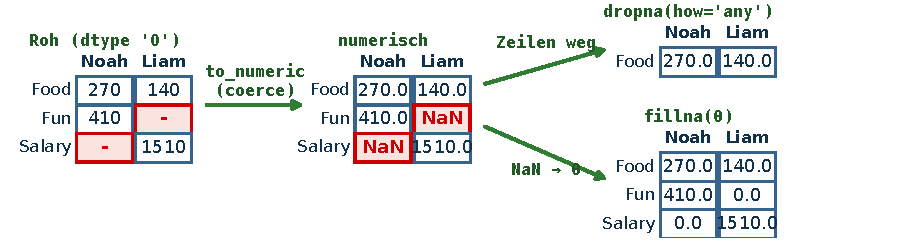
\includegraphics[width=\columnwidth]{Images/pandas-data-cleaning-missing-values-pipeline.pdf}
\end{center}
\end{contentbox}

\subsection{Auswerten}\label{sec:08-auswerten}
\subsubsection{Hilfsfunktionen für DataFrames}\label{sec:08-hilfsfunktionen-für-dataframes}
\begin{contentbox}
\CodeLine{data["Age"].sum()}[summiert alle Werte der Spalte `Age']\\
\CodeLine{data["Age"].max()}[maximaler Wert]
\end{contentbox}






%=====================================================================================================================
%%%%%%%%%%%%%%%%%%%%%%%%%%%%%%%%%%%%%%%
